\section{Color Polarization Filter Array Sensors}
In recent years, the development of microscopic polarization filters has enabled the production of camera sensors where each pixel has its own polarization filter, as illustrated in Figure \ref{fig:camera_crosstalk} \cite{lucidvisionlabsLUCIDGoingPolarizedWhitePaper2018}.
\begin{figure}[H]
    \centering
    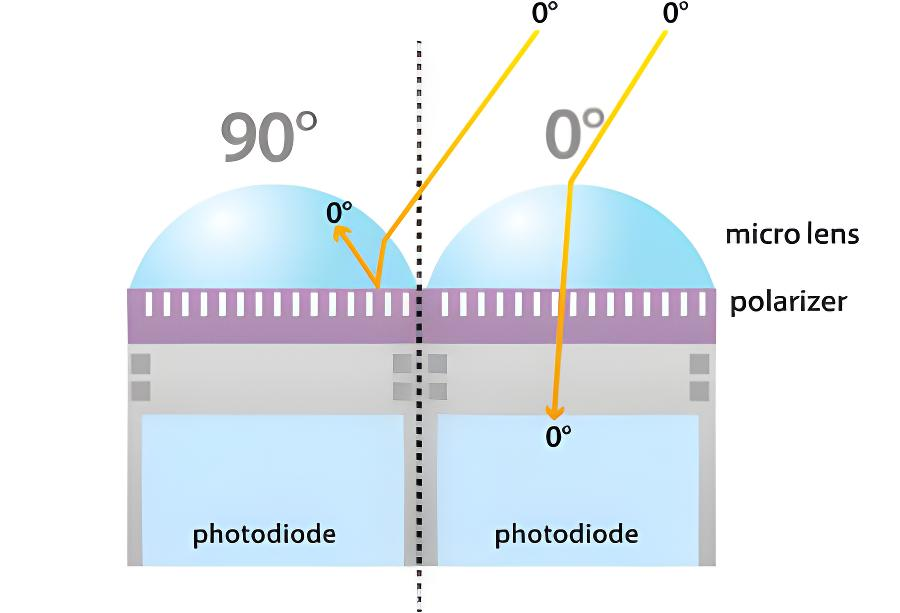
\includegraphics[width=0.48\textwidth]{figures/crosstalk_off_upscaled.jpg}
    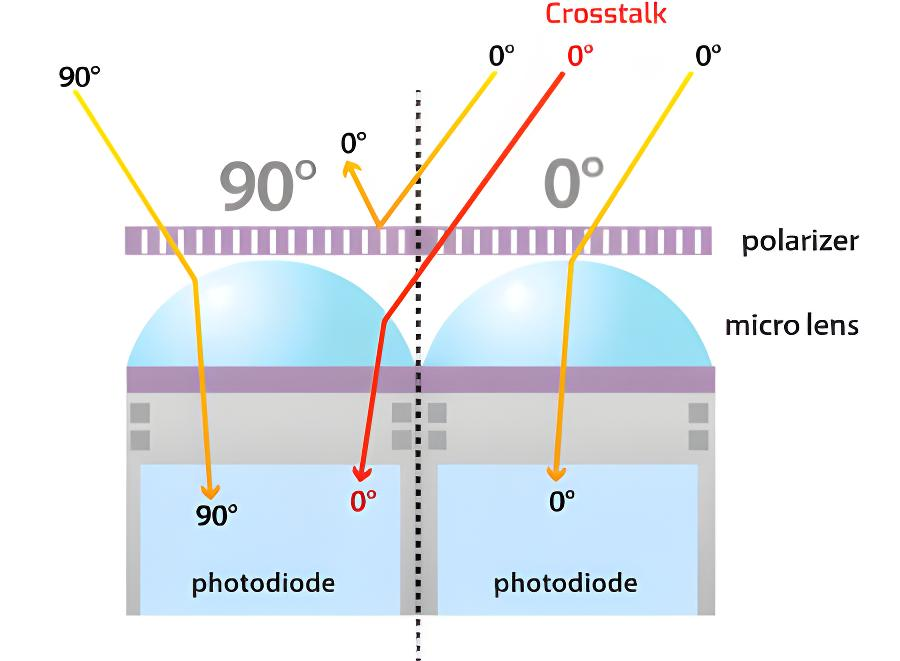
\includegraphics[width=0.48\textwidth]{figures/crosstalk_upscaled.jpg}
    \caption{Polarizer developed by Sony (left) to ensure low crosstalk between pixels \cite{lucidvisionlabsPolarizationExplainedSony2018}.}
    \label{fig:camera_crosstalk}
\end{figure}
\glspl{pg} can be formed from groups of four pixels with different filter angles, allowing the capture in practice to capture four pictures simultaneously with angles of polarization.
A Bayer Pattern can be added on top of this, resulting in groups of 16 pixels called \glspl{cpg}, enabling the capture of color information as well.
This configuration is referred to as a \gls{cpfa} and is illustrated in Figure \ref{fig:polarization_naming}.

\begin{figure}[H]
    \centering
    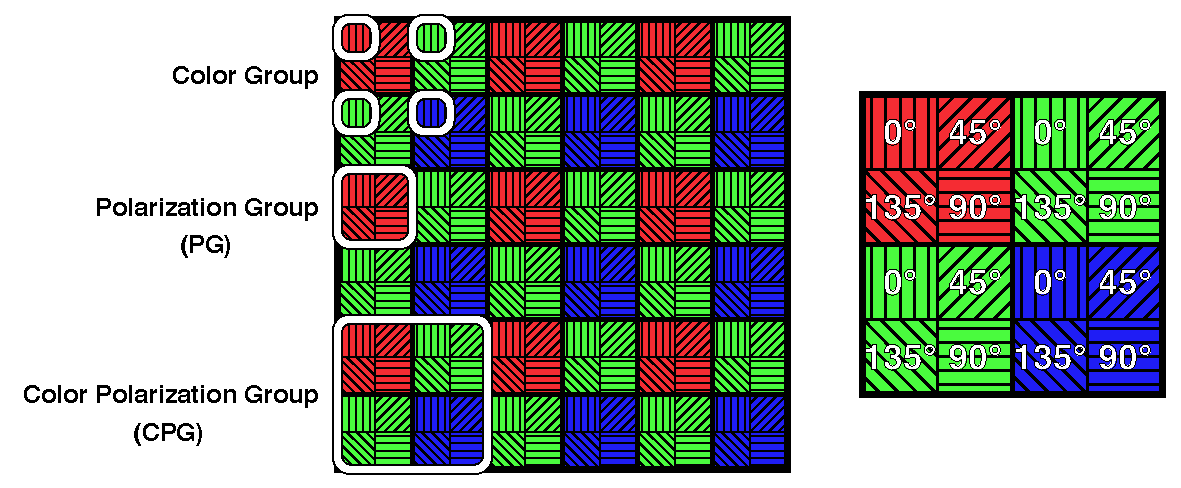
\includegraphics[width=\textwidth]{figures/polarized_image/naming.pdf}
    \caption{Naming convention for the different polarization angles.}
    \label{fig:polarization_naming}
\end{figure}

\subsection{Stokes Parameters}
Given the four polarisation angles, the Stokes parameters can be calculated \cite{piascoSurveyVisualBasedLocalization2018}.
With these parameters, the \gls{dolp} and \gls{aolp}, which is the angle of polarization relative to the camera, can be calculated as follows \cite{piascoSurveyVisualBasedLocalization2018}:
\begin{align}
    S_0 =  & I_0 + I_{90}                                                      \\
    S_1 =  & I_0 - I_{90}                                                      \\
    S_2 =  & I_{45} - I_{135}                                                  \\
    DoLP = & \frac{\sqrt{S_1^2 + S_2^2}}{S_0}  \label{eq:dolp}                 \\
    AoLP = & \frac{1}{2} \arctan{\left(\frac{S_2}{S_1}\right)} \label{eq:aolp}
\end{align}

A common way to visualize this is to encode the \gls{aolp} as hue and the \gls{dolp} as the value in the \gls{hsv} color space.
This can either be done for the three color channels separately or after calculating the grayscale value, which is illustrated in Figure \ref{fig:polarization_visualization}, which is captured by the \sr.
The benefits of polarization are evident in this image, as the water surface has a high \gls{dolp} and predictable \gls{aolp}.
The benefits and limitations of this polarization information are further discussed in Section \ref{sec:pol_benefits}.

\begin{figure}[H]
    \centering
    \subcaptionbox{The four polarization channels with $0^\circ$, $45^\circ$, $90^\circ$ and $135^\circ$ polarization angle respectively.}{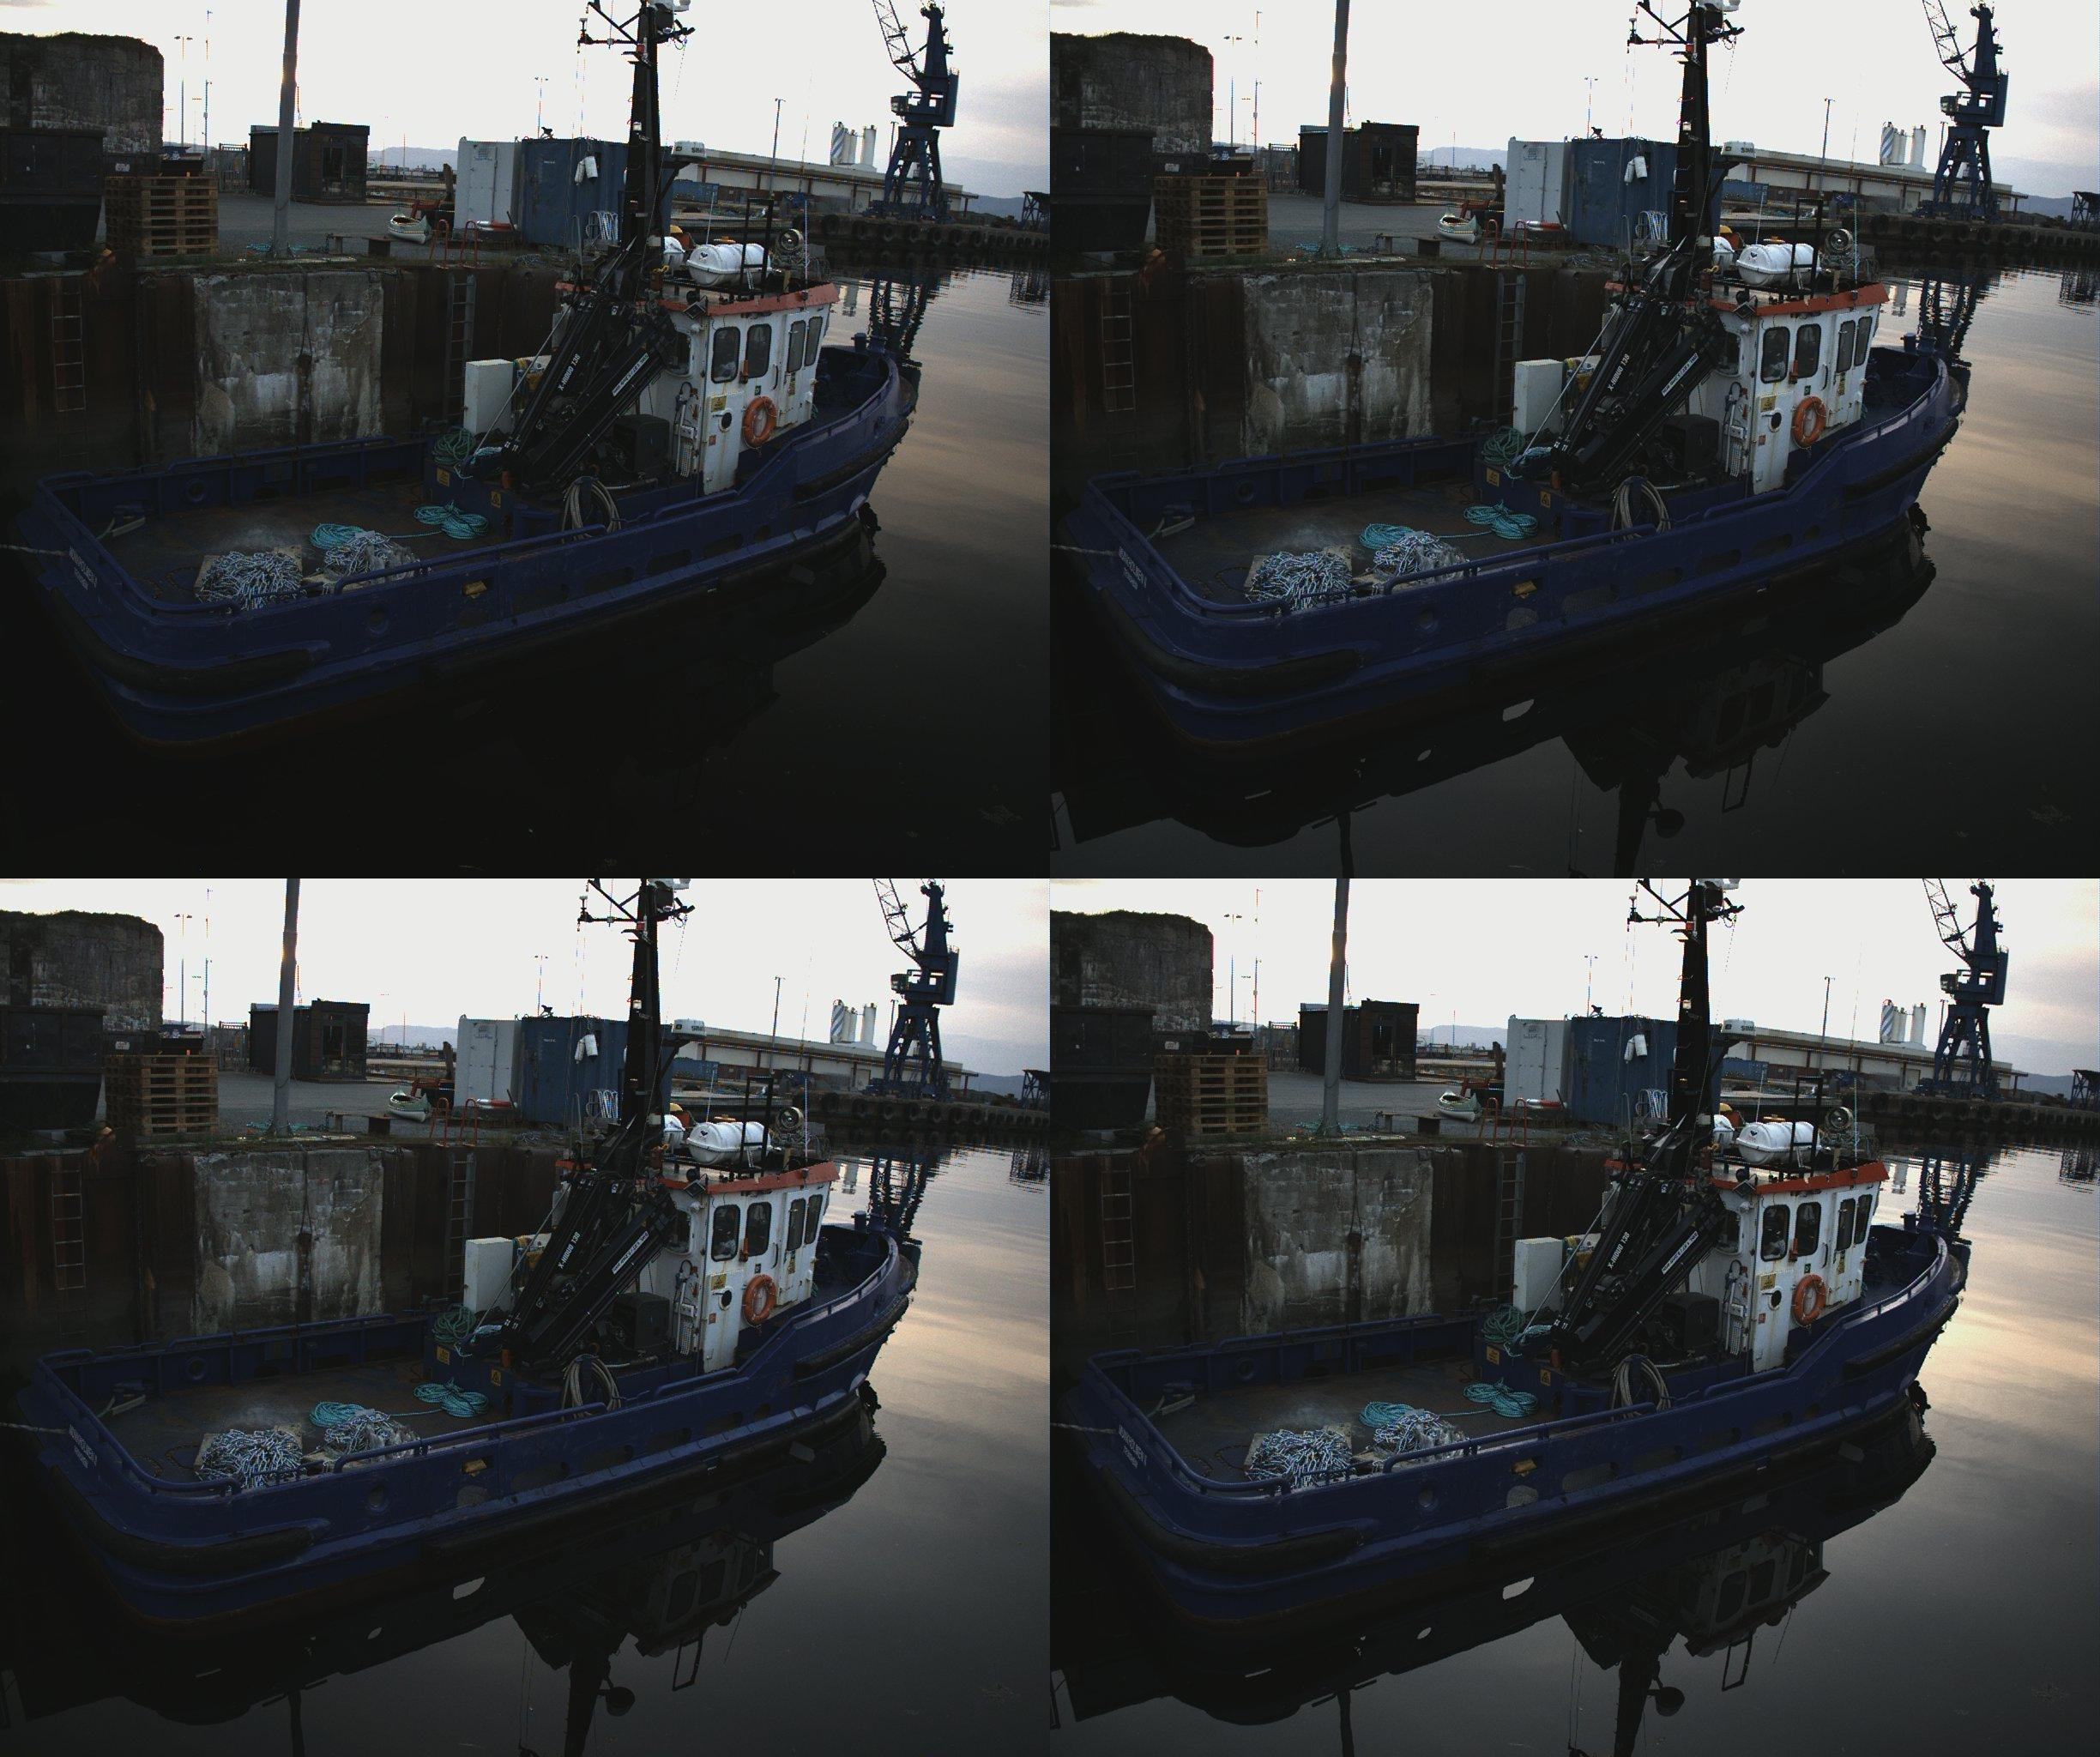
\includegraphics[width=.8\textwidth]{figures/pictures/img_00231_split.jpeg}}
    \subcaptionbox{\gls{aolp} and \gls{dolp} visualized as hue and value.}{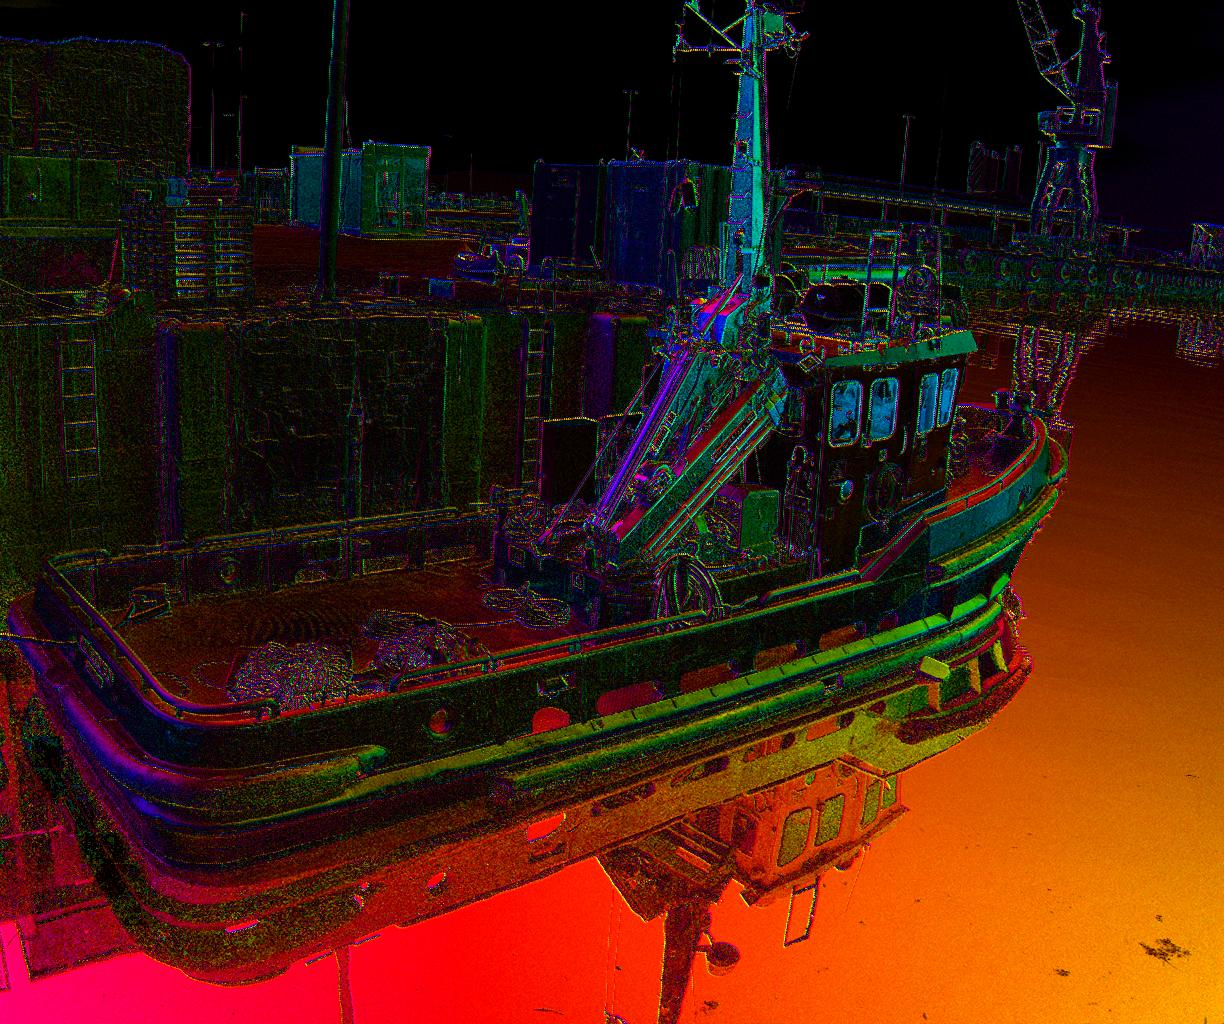
\includegraphics[width=.8\textwidth]{figures/pictures/aolp_left_231.jpeg}}
    \caption{Visualization of a \gls{cpfa} sensor.}
    \label{fig:polarization_visualization}
\end{figure}



